%%%%%%%%%%%%%%%%%%%%%%%%%%%%%%%%%%%%%%%%%
% PhD Thesis
% Cilie W. Feldager
%
% progplan: https://docs.google.com/spreadsheets/d/1w7HuOBZHn7flwv08kWuxVxPYJXr9nv2VGs3Gq5927qw/edit#gid=1834352503
%
% Based Jesper Rask Pedersen's thesis which was based on dionhaefner's thesis which was based on uiothesis and classicthesis
%
% Compile with ``pdflatex -shell-escape "thesis".tex``
%
% License:
% CC BY-NC-SA 3.0 (http://creativecommons.org/licenses/by-nc-sa/3.0/)
%
%%%%%%%%%%%%%%%%%%%%%%%%%%%%%%%%%%%%%%%%%

%-----------------------------------------------
%   PACKAGES AND OTHER DOCUMENT CONFIGURATIONS
%-----------------------------------------------

\documentclass[a4paper,12pt,twoside,blackthesis,openright]{phdthesis} % Other options draft, blackthesis


% Language setup
\usepackage[danish,english]{babel}
\setquotestyle{english}

%\hyphenation{pa-ra-me-te-ri-za-tion vis-cosi-ty sver-drups dions-thesis}
\graphicspath{{figures/\blackfigspath}} % appends to path if blackthesis is chosen
\bibliography{references.bib}
%\addbibresource{references.bib}

\usepackage{listings}

% Additional preamble files
%\input{preamble/pgfcache}
%%%
%% Code listings
%%

\usepackage[cache,chapter]{minted}
\usepackage[many,minted]{tcolorbox}
\usemintedstyle{friendly}

\newcommand{\listlistingsname}{List of Code Listings}
\renewcommand{\listingscaption}{Code Listing}
\newlistentry{listing}{lol}{0}
\renewcommand{\cftlistingleader}{ }
\renewcommand{\cftlistingafterpnum}{\cftparfillskip}

\newcommand{\mynewminted}[3]{%
	\newminted[#1]{#2}{#3}%
	\tcbset{myminted/#1/.style={minted language=#2,minted options={#3}}}}

\mynewminted{pythoncode}{python}{autogobble, linenos, xleftmargin=1em, python3}

\newtcblisting{listingsbox}[2][]{%
	listing only,enhanced,colback=black!3!white,%
	arc=0mm,frame hidden,myminted/#2,#1}

% see http://tex.stackexchange.com/questions/20890/define-an-escape-underscore-environment
\makeatletter
\DeclareRobustCommand*{\escapeus}[1]{%
	\begingroup\@activeus\scantokens{#1\endinput}\endgroup}
\begingroup\lccode`\~=`\_\relax
\lowercase{\endgroup\def\@activeus{\catcode`\_=\active \let~\_}}
\makeatother

\DeclareRobustCommand{\run}[1]{\texttt{\escapeus{#1}}}
\newcommand{\grid}[1]{\run{#1}}

\DefineBibliographyStrings{english}{%
	backrefpage = {Cited on p.~},
	backrefpages = {Cited on pp.~}
}


\newcommand{\meanchristoffel}[2]{\tilde{\Gamma}^{#1}_{\hphantom{#1}#2}}% Christoffel symbol
\newcommand{\varchristoffel}[2]{\hat{\Gamma}^{#1}_{\hphantom{#1}#2}}% Christoffel symbol

\newcommand{\K}{\mathbf{K}} % Covariance/kernel Matrix
\newcommand{\Y}{\mathbf{Y}} % Observations
\newcommand{\X}{\mathbf{X}} % Latents


%\renewcommand{\det}[1]{\operatorname{det}(#1)} % Determinant
\newcommand{\D}{\mathrm{d}} % Differential


\newcommand{\length}{\operatorname{Length}} % Length
\newcommand{\energy}{\operatorname{Energy}} % Energy

\newcommand{\cov}{\operatorname{cov}} % Covariance
\newcommand{\tra}{^{\top}} % Matrix transpose
\newcommand{\inv}{^{-1}} % Matrix Inverse
\newcommand{\Rcal}{\mathcal{R}} % Rest set
\newcommand{\Acal}{\mathcal{A}} % Active set
\newcommand{\N}{\mathcal{N}} % Normal
\newcommand{\Vcal}{\mathcal{V}} % Vietoris-Rips complex
\newcommand{\Ncal}{\mathcal{N}} % Normal
\newcommand{\Lcal}{\mathcal{L}} % Lower bound
\newcommand{\Dcal}{\mathcal{D}} % pbservations
\newcommand{\I}{\mathbb{I}} % Identity matrix
\newcommand{\Ibb}{\mathbb{I}} % Identity matrix
\newcommand{\Ebb}{\mathbb{E}} % Expectation
\newcommand{\GP}{\mathcal{GP}} % GP
\newcommand{\R}{\mathbb{R}} % Natural numbers
\newcommand{\Rbb}{\mathbb{R}} % Natural numbers
\newcommand{\M}{\mathcal{M}} % Manifold
\newcommand{\Mcal}{\mathcal{M}} % Manifold
\newcommand{\Wcal}{\mathcal{W}} % Wishart distribution
\newcommand{\Xcal}{\mathcal{X}} % Latent Space
\newcommand{\Ycal}{\mathcal{Y}} % Observation Space
\newcommand{\T}{\mathcal{T}} % Tangent space
\newcommand{\Tcal}{\mathcal{T}} % Normal
\newcommand{\KL}{\operatorname{KL}} % KL div
\newcommand{\s}{\sigma} % Sigma
%\newcommand{\trans}{^\top}}} % Tranpose
\newcommand{\christoffel}[2]{\Gamma^{#1}_{\hphantom{#1}#2}}% Christoffel symbol
\newcommand{\norm}[1]{\left\lVert#1\right\rVert} % Norms
\newcommand{\dydx}[2]{\frac{\partial{#1}}{\partial{#2}}} % Partial derivatives
\newcommand{\dydxsquared}[2]{\frac{\partial^2{#1}}{\partial{#2} ^2}} % Partial derivatives
\newcommand{\jac}{\mathbf{ J}} %Jacobian
\newcommand{\J}{\mathbf{J}} %Jacobian
\renewcommand{\vec}[1]{\mathbf{#1}} % Vector





\renewcommand{\eqref}[1]{equation~\ref{#1}}
\newcommand{\Eqref}[1]{Equation~\ref{#1}}
\newcommand{\partref}[1]{part~\ref{#1}}
\newcommand{\Partref}[1]{Part~\ref{#1}}
\newcommand{\figref}[1]{figure~\ref{#1}}
\newcommand{\Figref}[1]{Figure~\ref{#1}}
\newcommand{\tabref}[1]{table~\ref{#1}}
%\newcommand{\secref}[1]{\textsection\,\ref{#1}}
\newcommand{\secref}[1]{section~\ref{#1}}
\newcommand{\Secref}[1]{Section~\ref{#1}}
\newcommand{\thref}[1]{theorem~\ref{#1}}
\newcommand{\Thref}[1]{Theorem~\ref{#1}}
\newcommand{\chapref}[1]{chapter~\ref{#1}}
\newcommand{\Chapref}[1]{Chapter~\ref{#1}}
\newcommand{\appendixref}[1]{appendix~\ref{#1}}
\newcommand{\Appendixref}[1]{Appendix~\ref{#1}}
\newcommand{\listingref}[1]{code~listing~\ref{#1}}


\MakeRobust{\eqref}
\MakeRobust{\figref}
\MakeRobust{\Figref}
\MakeRobust{\partref}
\MakeRobust{\Partref}
\MakeRobust{\eqref}
\MakeRobust{\Eqref}
\MakeRobust{\tabref}
\MakeRobust{\thref}
\MakeRobust{\Thref}
\MakeRobust{\chapref}
\MakeRobust{\Chapref}
\MakeRobust{\appendixref}
\MakeRobust{\Appendixref}
\MakeRobust{\listingref}

\newcommand{\gp}{Gaussian process}
\newcommand{\gps}{Gaussian processes}
\newcommand{\gplvm}{Gaussian process latent variable model}

\newcommand{\pla}{principle of least action }
\newcommand{\wrt}{with respect to }
\newcommand{\ie}{i.\,e., }
\newcommand{\Ie}{I.\,e., }
\newcommand{\eg}{e.\,g.\ }
\newcommand{\Eg}{E.\,g.\ }
\newcommand{\cf}{cf.\ }
\newcommand{\Cf}{Cf.\ }

\newcommand{\rn}[1]{%
	\textup{\uppercase\expandafter{\romannumeral#1}}%
}

\newcommand{\orderof}[1]{\mathcal{O}\left(#1\right)}
\newcommand{\curl}{\text{curl}}
\newcommand{\divergence}{\text{div}}
\newcommand{\dx}[1]{~\text{d}#1}
\newcommand{\Ddx}[1][]{\frac{\text{D}#1}{\text{d}t}}
\newcommand{\mean}[1]{\langle #1 \rangle}
\newcommand{\abs}[1]{\left| #1 \right|}
\newcommand{\updel}{\mathop{}\!\upDelta}

\DeclareSIUnit\sv{Sv}
\DeclareSIUnit\year{y}
\DeclareSIUnit\permille{\text{\textperthousand}}

\newcommand{\oldand}{\textsw{\& }}
\newcommand{\work}[1]{\textsw{#1}}

\DeclareFieldFormat*{citetitle}{\work{#1}}
\newcommand{\citebook}[1]{\citetitle{#1} \citep{#1}}



\newcommand{\documenttype}{Ph.D. Thesis}
\newcommand{\thesistitle}{Statistics under Stochastic Metrics}
\newcommand{\thesisauthor}{Cilie W. Feldager} % Your name :) 
\newcommand{\universityname}{Technical University of Denmark}
\newcommand{\department}{DTU Compute}
\newcommand{\departmentdescriber}{Department of Applied Mathematics and Computer Science}
\newcommand{\sectionname}{Cognitive Systems}


\newcommand{\addressI}{Richard Petersens Plads, Building 321}
\newcommand{\addressII}{2800 Kgs. Lyngby}
\newcommand{\phonenumber}{Phone +45 4525 1700}
\newcommand{\departmentwebsite}{www.compute.dtu.dk}
 % Info on author, uni, etc
%%%%%%%%%%%%%%%%%%%%%%%%%%%%%%%%%%%%
% draft packages, remove for final version
\usepackage{todonotes}
\newcommand{\firstdraft}[1]{\todo[inline,color=green!20!white]{\textbf{\thesubsection \ First draft} #1}}
\newcommand{\why}[1]{\todo[inline,color=purple!80!white]{\textbf{\thesubsection \  Question:} #1}}
\newcommand{\dado}[1]{\todo[inline,color=red!20!white]{\thesubsection \ \textbf{Do:} #1}}

\newcommand{\nice}[1]{\todo[inline,color=dtugreen!80!white]{\thesubsection \ {\color{white}\textbf{Nice to have: #1} #1}}}
\newcommand{\need}[1]{\todo[inline,color=red!80!white]{\thesubsection \ \textbf{Need to have:} #1}}

\newcommand{\experiment}[1]{\todo[inline,color=blue!70!white]{{\color{white}\thesubsection \ \textbf{Experiment:} #1}}}

\newcommand{\sanity}[1]{\todo[inline,color=gray!80!white]{\thesubsection \ {\color{gray}\textbf{Sanity check:} #1}}}
\newcommand{\soren}[1]{\todo[inline,color=purple!80!white]{\thesubsection \ \textbf{Søren: } #1}}
\newcommand{\jesper}[1]{\todo[inline,color=blue!20!white]{\thesubsection \ \textbf{Jesper:} #1}}
\newcommand{\pablo}[1]{\todo[inline,color=yellow!80!white]{\thesubsection \ \textbf{Pablo:} #1}}

\newcommand{\done}[1]{\todo[inline,color=green]{\thesubsection \ \textbf{Done} #1}}
\newcommand{\howto}[1]{\todo[inline,color=blue!20!white]{\thesubsection \  \textbf{How to} #1}}
\newcommand{\remember}[1]{\todo[inline,color=pink!80!white]{\thesubsection \  \textbf{Remember} #1}}

%\definecommand{sectiontitle}{#1}
%\definecommand{setsectiontitle}[1]{\renewcommand{sectiontitle}{#1}}
%\newcommand{\sectiontitle}{}
%\newcommand{\newsection}[1]{\section{#1}\renewcommand{\sectiontitle}{#1}}
%\newcommand{\subsectiontitle}{}
%\newcommand{\newsubsection}[1]{\subsection{#1}\renewcommand{\subsectiontitle}{#1}}

%\usepackage{showlabels}
\usepackage{tcolorbox}
\usepackage{blindtext}
\usepackage{lipsum}

  % Draft packages. This line can be outcommented when done

\usepackage{makeidx}
\makeindex

\hyphenation{co-vector}

% Don't know what these do, outcomment on 2022-06-22
%\usepackage[acronym,automake]{glossaries-extra}
%\setabbreviationstyle[acronym]{long-short}
%\newacronym{gplvm}{GP-LVM}{Gaussian process latent variable model}
%\newacronym{dtu}{DTU}{Technical University of Denmark}
%\makeglossaries

\usepackage[font=small,skip=5pt]{caption}

%\usepackage{nomencl}
%\makenomenclature

%%%%%%%%%%%%%%%%%%%%%%%%%%%%%%%%%%%%
% Stuff that should be moved at a later point
% Should be moved to class

% MATH STUFF
\usepackage{algorithm}
\usepackage{algorithmic}

%\usepackage{lastpage} % lastpage, commented out on 04.JUN because I don't know what it does.
\usepackage{amsmath,amssymb,mleftright} % amsmath&symboler

\usepackage{cleveref}
\crefname{part}{part}{parts}
\crefname{chapter}{chapter}{chapters}
\crefname{section}{section}{sections}
\crefname{subsection}{subsection}{subsections}

% Used for the table in example.tex
\usepackage{booktabs} 
%\usepackage{siunitx} % for having numbers aligned to the decimal point
\usepackage{array}
\newcolumntype{L}[1]{>{\raggedright\arraybackslash}p{#1}}

\usepackage{morewrites} % Fixes something I don't quite understand but I added it myself. Test if it is needed. Keep it in for now (2021-04-27). I had removed it in may-2022 and ended up debugging a bunch to realise that I need this package!

% Change the appearance of margin notes
\renewcommand*{\marginfont}{\footnotesize}

\usepackage{amsmath} % provides numberwithin (and lots more)
\newtheorem{theorem}{Theorem}[chapter]
\newtheorem{definition}{Definition}[chapter]
\newtheorem{remark}{Remark}%[chapter]

\usepackage{listlbls}


\usepackage[final]{pdfpages}
\usepackage{tikz}
\usetikzlibrary{bayesnet}
\usetikzlibrary{arrows}

\usepackage{forest}
\usepackage{cancel}

\definecolor{folderbg}{RGB}{124,166,198}
\definecolor{folderborder}{RGB}{110,144,169}

\def\Size{4pt}
\tikzset{
  folder/.pic={
    \filldraw[draw=folderborder,top color=folderbg!50,bottom color=folderbg]
      (-1.05*\Size,0.2\Size+5pt) rectangle ++(.75*\Size,-0.2\Size-5pt);  
    \filldraw[draw=folderborder,top color=folderbg!50,bottom color=folderbg]
      (-1.15*\Size,-\Size) rectangle (1.15*\Size,\Size);
  }
}


%%%%%%%%%%%%%%%%%%%%%%%%%%%%%%%%%%%%
% define bools for handy include of front-, main- and back matters
\newboolean{includefrontmatter}   
\newboolean{includemainmatter}   
\newboolean{includebackmatter}   

%%%%%%%%%%%%%%%%%%%%%%%%%%%%%%%%%%%%
%%%%%%%%%%%%%%%%%%%%%%%%%%%%%%%%%%%%
%%%%%%%%%%%%%%%%%%%%%%%%%%%%%%%%%%%%
\begin{document}
%%%%%%%%%%%%%%%%%%%%%%%%%%%%%%%%%%%%

\setboolean{includefrontmatter}{true}   
\setboolean{includemainmatter}{true}   
\setboolean{includebackmatter}{true}   

%\pagestyle{simple}
% Setting the style of the chapter
%\chapterstyle{mychapterstyle} % uses images instead of actual numbers. Make sure that these images are the same size and that enough of them correspond to the number of chapters. You should have a set for both black and white thesis
\chapterstyle{margin} 


% I have no clue why this should be necessary. I want to delete it.
% check alphabet length
%\newlength{\alphabetlength}
%\settowidth{\alphabetlength}{abcdefghijklmnopqrstuvwxyz}
%\the\alphabetlength
%-----------------------------------------------
%   FRONT MATTER
%-----------------------------------------------

\ifthenelse{\boolean{includefrontmatter}}{ % start of bool to include frontmatter

\frontmatter
\pdfbookmark[-1]{Front matter}{frontmatter}
\pagestyle{empty}
\pagenumbering{gobble}
\hypersetup{pageanchor=false}

\pagecolor{coverbackgroundcolor}
\color{covertextcolor}

\begin{whole}
	\centering

	{\begin{tabular}{p{\linewidth}}
		\vspace{0.5cm}
		{\hspace{-1.9cm}\HUGE \spacedlowsmallcaps \thesistitle}   \bigskip \\ 
		\hspace{-1.9cm}\spacedlowsmallcaps{\Large\sffamily \thesisauthor}\\
		{\hspace{-1.9cm}\spacedlowsmallcaps{\Large\sffamily \documenttype}}
	\end{tabular}}
	
	\begin{tikzpicture}[remember picture,overlay]
		\node[anchor=north east, xshift=-10mm, yshift=-12mm] 
		at (current page.north east) 
     		{\color{covertextcolor}
       		 \begin{tabular}{r} 
			\textbf{\spacedlowsmallcaps \department} \\ 
        			\spacedlowsmallcaps \departmentdescriber
        		\end{tabular}
      		}; 
	\end{tikzpicture}
		
	% DTU logo
	\begin{tikzpicture}[remember picture,overlay]
		\node[anchor=north west, xshift=8.9mm, yshift=-8.3mm] 
	    	 at (current page.north west) 
		{
\includegraphics[width=14.75mm,keepaspectratio]{logo.pdf}};
	\end{tikzpicture}

	
	% Cover photo
	\begin{tikzpicture}[remember picture,overlay]
%		\node[anchor=south, xshift=0pt, yshift=-70mm] at (current page.south)
%	     	{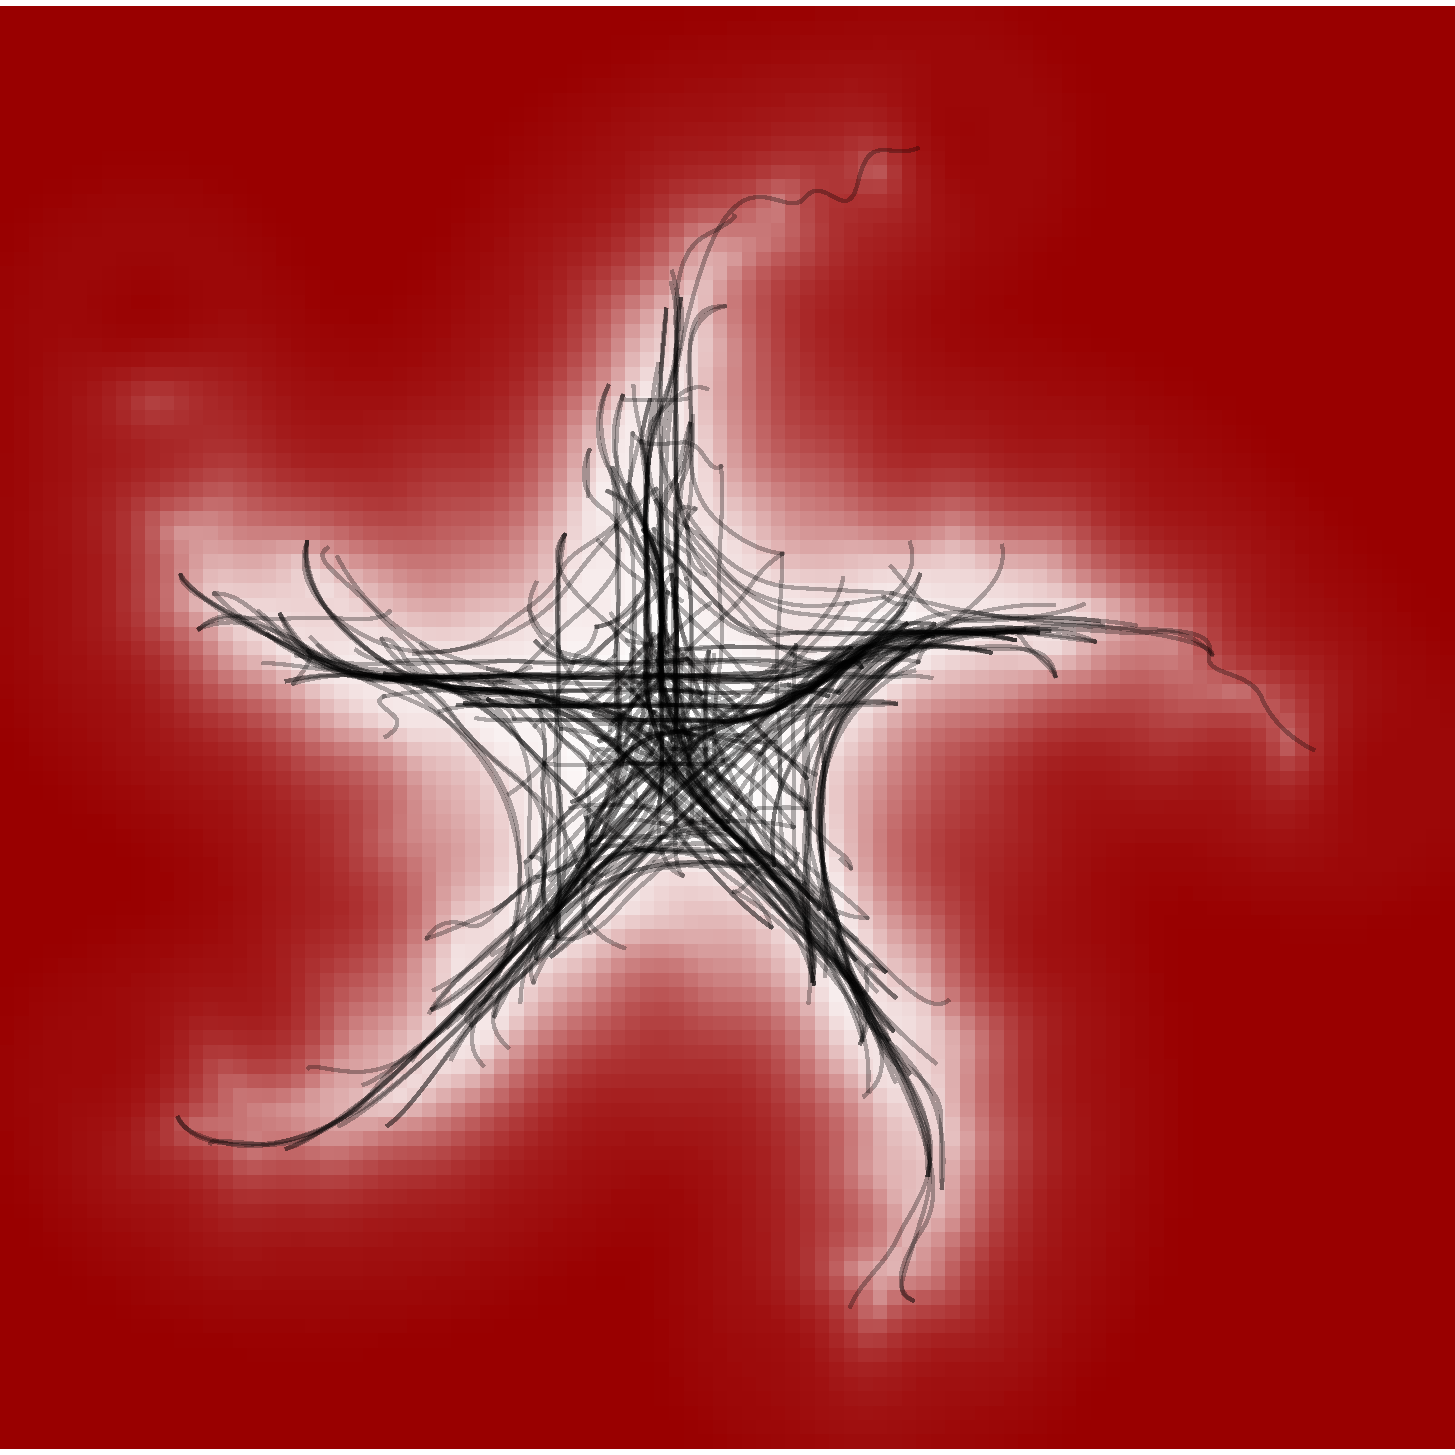
\includegraphics[height=30.5cm,keepaspectratio]{frontpage.pdf}};
		\node[anchor=south, xshift=0pt, yshift=-2.5mm] at (current page.south)
	     	{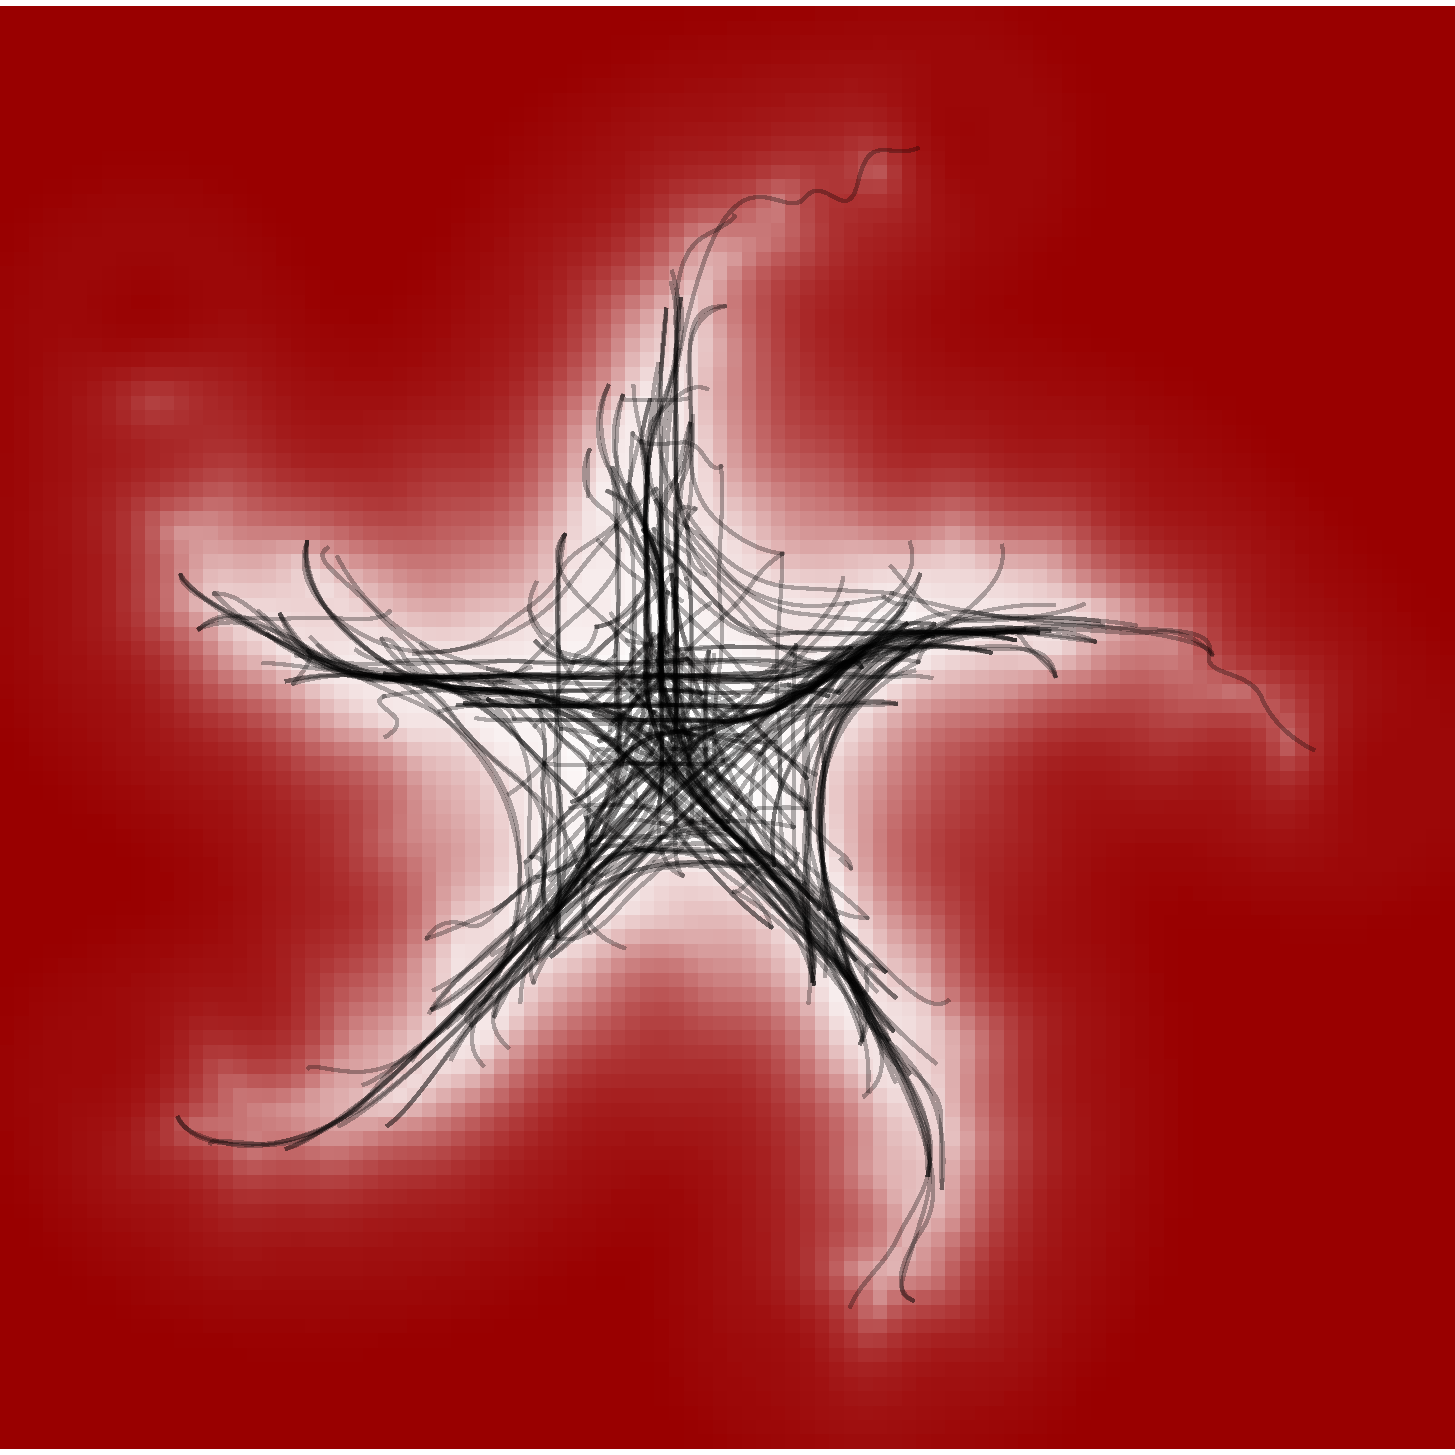
\includegraphics[width=\paperwidth,keepaspectratio]{frontpage.pdf}};		
		
	\end{tikzpicture}
	
\end{whole}

\clearpage
\pagecolor{pagecolor}
\color{textcolor}
%TODO:  \color{covertextcolor} Need to set the pagecolor back to white
\cleardoublepage


\begin{whole}
	\begin{center}
		%\hspace{-2cm}{\color{largeornament}\fourierOrnament{100}{120}{97}}
		\vspace*{5cm}\hspace{-2cm}{\color{smallornament}\fourierOrnament{100}{120}{93}}
		% 90-93,97-100,102-104

		%\hspace{-2cm}{\color{largeornament}\floweroneright}%{100}{120}{97}}
		
		
	\end{center}
\end{whole}

\vspace*{\fill}

\sfcaps{\documenttype} \\
\sfcaps{\thesistitle}\\
\sfcaps{By \thesisauthor}

\vspace{2ex}

\noindent \sfcaps{\sectionname}\\
\sfcaps{\department}\\
\sfcaps{\universityname}

\vspace{2ex}

\sfcaps{Supervised by} \\
\sfcaps{Professor S\o ren Hauberg}\\
%and\\[.8em]
\sfcaps{Professor Lars Kai Hansen}
%\vspace{3em}



\cleardoublepage
\cleardoublepage

%\pagenumbering{roman}
%\pagestyle{simple}
%
%\include{frontmatter/dedication}
%\cleardoublepage
%
%\include{frontmatter/abstract}
%\cleardoublepage
%
%\include{frontmatter/abstract_danish}
%\cleardoublepage
%
%\include{frontmatter/preface}
%\cleardoublepage
%
%\include{frontmatter/acknowledgements}
%\cleardoublepage
%
%%*******************************************************
% List of publications
%*******************************************************
\refstepcounter{dummy}
\pdfbookmark[1]{List of Publications}{listofpublications}

%\null
%\vspace{4\onelineskip}

%\fancyquote{Isaac Newton}{%
%    If I have seen further, it is by standing on the shoulders of giants.
%}

%\vspace{2\onelineskip}

\begingroup
\let\clearpage\relax

\section*{List of Publications}
Pablo Moreno-Mu\~{n}oz*, Cilie W. Feldager*\marginnote{* Equal contribution}, and Søren Hauberg \\ \textit{Revisiting Active Sets for Gaussian Process Decoders}. Sept. 2022.
\\ \textsc{DOI}:10.48550/arXiv.2209.04636.arXiv:2209.04636 [cs, stat]
\\ Poster at Neural Information Processing Systems, 2022.

\vspace{1cm}
Cilie W. Feldager, Søren Hauberg, and Lars Kai Hansen.\\  \textit{Spontaneous Symmetry Breaking in Data Visualization}.\\ In: Artificial Neural Networks and Machine Learning. \\
Lecture Notes in Computer Science (Including Subseries Lecture Notes in Artificial Intelligence and Lecture Notes in Bioinformatics)".
Springer, 2021, pp. 435–446. isbn: 978-3-030-86339-5.\\
\textsc{DOI}: 10.1007/978-3-030-86340-1\_35


\endgroup
%\cleardoublepage

%*******************************************************
% Table of Contents
%*******************************************************
\refstepcounter{dummy}
\pdfbookmark[1]{\contentsname}{tableofcontents}
\thispagestyle{simple}
\tableofcontents*
%\clearpage
\cleardoublepage


%*******************************************************
% List of Figures, Tables, Listings, Acronyms, Notation
%*******************************************************

\begingroup 

%*******************************************************
% List of Figures
%*******************************************************  
%\refstepcounter{dummy}
%\pdfbookmark[1]{\listfigurename}{lof}
%\newlistof{listoffigures}{lof}{\listfigurename}
%\listoffigures*
%
%\clearpage
%\cleardoublepage

%*******************************************************
% List of Tables
%*******************************************************
%\refstepcounter{dummy}
%\pdfbookmark[1]{\listtablename}{lot}
%\newlistof{listoftables}{lot}{\listtablename}
%\listoftables*

%\vspace*{2.5cm}
%*******************************************************
% List of Listings
%*******************************************************      
%\refstepcounter{dummy}
%\pdfbookmark[1]{\listlistingsname}{lol}
%\newlistof{listoflistings}{lol}{\listlistingsname}
%\listoflistings*
%
%%\clearpage

%\cleardoublepage

%*******************************************************
% Acronyms
%*******************************************************
\iffalse
\refstepcounter{dummy}
\pdfbookmark[1]{Acronyms}{acronyms}
\chapter*{Acronyms}
\dado{sort alphabetically, update if needed or simply delete}
\begin{acronym}[NGCUCX]
	\acro{GP}{Gaussian Process}
	\acro{GPLVM}{Gaussian Process Latent Variable Model}
	\acro{PCA}{Principal Component Analysis}
	\acro{PPCA}{Probabilistic Principal Component Analysis}	
	\acro{kPCA}{Kernel Principal Component Analysis}
	\acro{SNE}{Stochastic Neighbourhood Embedding}
	\acro{t-SNE}{t-Distributed Stochastic Neighbourhood Embedding}
	\acro{MF}{Magnification Factor}
	\acro{Adam}{Adaptive Moment Estimation}
	\acro{VAE}{Variational Autoencoder}
	\acro{NN}{Neural Network}
	\acro{SAS}{Stochastic Active Sets}
	\acro{POLA}{Principle of Least Action}
\end{acronym}   
\fi
\iffalse
%*******************************************************
% Notation
%*******************************************************  
\refstepcounter{dummy}
\pdfbookmark[1]{Notation}{notation}
\chapter*{Notation}
\todo[inline]{Create table of notation for both Gp stuff and geometry stuff. This way I can make sure things are aligned.}
\section*{General}
$N$ is the number of observations \\
$D$ is the dimensionality of one observation/of data space/of the observed space \\
$q$ is the dimensionality of the latent space \\
$Y$ is data, this lives in the observed space so $Y \in \mathbb{R}^{N\times D}$, alternatively for one point we have $y_i \in \mathbb{R}^{D}$ \\
$X$ is a latent representation of data, this lives in the latent space so $X \in \mathbb{R}^{N\times D}$, alternatively for one point we have $y_i \in \mathbb{R}^{D}$ \\
We use $f$ to denote a map from the latent space to the bserved space such that $f: \mathbb{R}^q \to \mathbb{R}^D$ with $q < D$\\
$k(x,x')$ denotes the kernel that provides the covariance function. \\

I will denote derivatives in a number of ways. \marginnote{As we say in Danish, "dear child has many names}



\section*{GP}


\section*{Geometry}
Manifold \\
Tangent space \\
Curve \\
Christffel symbol \\
Uses Einstein notation \\

%\clearpage
\cleardoublepage
\fi


\endgroup % See also notation.tex
\cleardoublepage
}{}  % end of bool to include frontmatter




%-----------------------------------------------
%   MAIN MATTER
%-----------------------------------------------	
\ifthenelse{\boolean{includemainmatter}}{ % start of bool to include mainmatter

\mainmatter
\pagestyle{mystyle}
\bookmarksetup{startatroot}
\pagenumbering{arabic}
\hypersetup{pageanchor=True}
%\addtocontents{toc}{\protect\setcounter{tocdepth}{1}}

%\listoftodos

%-----------------------------------------------
%   BODY
%-----------------------------------------------

\pagestyle{mystyle}
\notocchapter{Documentation of class}
\label{chap:doc}


\fancyquote{Euclid}{That, if a straight line falling on two straight lines makes the interior angles on the same side less than two right angles, the two straight lines, if produced indefinitely, meet on that side on which the angles are less than two right angles.}


This class allows for typesetting a beautiful thesis with a few custom options. This chapter documents and displays the options in this class I implemented. Feel free to make it your own.

It builds on two other classes, Jesper's and Dion's which is build ono ?? and uses the principles from \texttt{Trees, maps, and theorems} by Jean-Luc Dumont (see section \ref{sec:trees}). Ultimately this are build on \texttt{memoir}. This can be used fr any type oof document.

\section{Main.tex}

For convenience, I introduced booleans that control if frontmatter, main matter or backmatter should be compiled. This is handy when having with numerous input files but working only in one.

\subsection{Blackthesis}
The \texttt{blackthesis} is an option parsed in the document class, eg \texttt{\textbackslash documentclass[a4paper,11pt,twoside,openright,blackthesis]\{phdthesis\}}. It changes the papercolor, textcolor, and link-,cite-,url colors. It always changes the figures path by appending a \texttt{blackfigs} to it. This means that a whole new set of figures are used to provide the user with both options.

The cover and back pages are likewise changed to match the \texttt{blackthesis} option and it allows for matching cover images.

The colors can be configured in the \textsc{phdthesis.cls}


\section{Preamble}
The directory preamble consists of four files. I inherited Listing.tex and misc.tex and I added drafts.tex and misc.tex myself.

\subsubsection{misc.tex}
Define handy shorthand commands for math and latex variables. This is handy for quickly changing the appearance/notation in a quick and consistent way.

\subsubsection{draft.tex}
\texttt{draft.tex} is a bunch of draft package like \texttt{todonotes} that allows for missingfigures, margin notes and inline notes. These can then be viewed in the todolist which is sort of like a table of contents for todos.


Having these in a separate file that can be commented out at the time of final compilation should ensure that no todos or blindtext can be left in the final document without raising errors.

\subsubsection{Figures}
If you know that you will have a figure of something, it can often be handy to include a placeholder. This can be done with the missing figure command \textbackslash\texttt{missingfigure} or the includegraphics command using a placeholder, \textbackslash\texttt{\textbackslash includegraphics[width=\textbackslash linewidth]\{example-image-golden\}}.




\subsection{statics.tex}
This file contains the information on the front and back pages. The information here is used in the file \textsc{frontmatter/frontpage.tex} (described in section \ref{frontpage}) and in  \textsc{backmatter/backpage.tex} (described in section \ref{backpage}) 

This is implemented an official DTU template that I don't recall where I found.


\section{Frontmatter}
Here one could add: Dedication, abstracts, acknowledgements, notation, preface, list of publications, acronyms, etc.

\subsection{frontpage.tex} \label{frontpage}
Adjust as you please

\subsection{contents.tex}
Contains toc, list of figs, notation, 

\section{Backmatter}
Thos could contains: Appendices, bibliographies, colophon (extra last page), publications.

Note that the blackoption might not work too well with inputting pdfs. You would probably have to manually set the background color of the page for these page. You can use the color names defined in the .cls to keep it dynamic.


\subsection{backpage.tex} \label{backpage}
Text can be added here to describe the project.



\subsection{A bit about references} \label{ssec:refs}
The reference can be set up in the class file.

The usual ref command gives: \ref{chap:intro}, \ref{sec:titles} and  \ref{ssec:refs}. But in the misc file, we define special reference commands for each depth that includes the prefix: \chapref{chap:intro}, \secref{sec:titles} and  \secref{ssec:refs}.

Likewise, we define other robust reference. The command can be seen below.
\begin{lstlisting}
\newcommand{\partref}[1]{Part \ref{#1}}
\newcommand{\figref}[1]{Fig.\ \ref{#1}}
\newcommand{\tabref}[1]{Table \ref{#1}}
\newcommand{\secref}[1]{\textsection\,\ref{#1}}
\newcommand{\chapref}[1]{Chapter \ref{#1}}
\newcommand{\appendixref}[1]{Appendix \ref{#1}}
\newcommand{\listingref}[1]{Code Listing \ref{#1}}
\end{lstlisting}

There are backreferences for the citations.



%%%%%%%%%%%%%%%%%%%%%%%%%%%%%%%%%%%
%%%%%%%%%%%%%%%%%%%%%%%%%%%%%%%%%%%
%%%%%%%%%%%%%%%%%%%%%%%%%%%%%%%%%%%
\notocchapter{My writing process}
I leave my brief thoughts on my writing process.


\section{The Braindump}
Hopefully, throughout my time as a student I have been doing some work. Writing papers, notes for yourself, code, making plots. Collect these. Group them.

\section{The Outline}
Based on the groups. Try to create a coherent stoory that include all of your groups. This might not be the chronological you did the work. Use bullets, and figures. Now what should go in each chapter, section, subsection and paragraph.

Discuss this with my supervisor. It is a lt easier to adjust things now rather than once I have finished all of the writing.

\section{The Vomit Draft}
Get the thoughts out of you head and onto paper. It is so much easier to edit than to start from a blank page. 

\section{Trees maps and theorems} \label{sec:trees}
Meta: This summarises this book in very short.

This class is built on \href{https://www.principiae.be/book/}{this book} by Jean-Luc Dumont\sidenote[-2]{It treats diffrent aspects of scientific coommunicationo but here we focus on written documents}. It defines three laws
\sidedef{First law}{}{
$$\textbf{Adapt to your audience}$$
}
My audience is first and foremost my committee. Next, I would like if master and Ph.D students might benefit from reading certain parts of the thesis. In either case I find it important to write in a style so I myself would have been able to understand at the beginning of my PhD studies. This is my starting point. With that being said, I have been more thorough or gone to a lower level in the part on geometry than for my own work. My intention is that the geometry chapter might be used for learning the elemental differential geometry needed for manifold learning using Einstein notation.

\sidedef{Second law}{}{
$$\textbf{Maximize the signal-to-noise ratio}$$
}
Tried doing this by not going into too much detail on methods that I expect people to know. I also have a matetext at the beginning of each part, chapter and section that explain the aim of the writing. I have tried following Tara Brabazon's ideas about topic sentences and the paragraph which lead me to develop a certain structure for each paragraph, see more on this in section \ref{sec:theparagraph}

\sidedef{Third law}{}{
$$\textbf{Use effective redundancy}$$
}
\todo[inline,color=mypink]{Read \href{https://www.principiae.be/book/pdfs/TM&Th-2.0-summary.pdf}{this summary} again}


\section{The paragraph} \label{sec:theparagraph}
Topic sentence, bridge sentence, template for a paragraph, one idea per paragraph. Link to Tara.

Tips:
1. Construct a strong, clear topic sentence.
The topic sentence should identify the main point of your paragraph. As a general rule, topic sentences should be clear enough that a reader can get the gist of your paper just by reading the topic sentences of each paragraph. Try to keep topic sentences simple (e.g., avoid breaking them up with commas). Once you’ve written your paragraph, it’s helpful to go back and check that a) you have a topic sentence, and b) it clearly captures the focal point of the paragraph.

2. Each paragraph should make one main point. In general, try to keep paragraphs between 3-5 sentences. If your paragraph is getting too long, it is probably making more than one main point, and it may be time to break it into two (and make a new topic sentence).

Main idea: ...
Old info: The manifold assumption is age old and use for justifying a lot of research. I
New info: Another way to put this into use is to exploit/compute the geometry explicitly by learning the metric and computing geodesics

Gaussian processes are considered too smooth and therefor does not capture the geometry.




3. Establish internal flow by placing old information first and new information last.






\section{Sanity checks}
This is a list of my sanity check, I would have liked to go through before submitting. I leave it here as it might be useful to someone else.

\begin{itemize}
\item All figures, tables, definitions, etc are referred to
\item All citations work, no ??
\item All references work, no ??
\item All figures have a label
\item All figures should have a short name
\item All figures should be placed properly, especially marginfigures. antimjustification is needed.
\item Clearly state what is my work/contributions/novelty
\item Check that all acronyms are added to the Acronyms
\item Check that everything is added the index
\item Check that no todos or example images or missing figures remain
\item Check for consistent notation
\item Check that notation page is up to date
\item Check that color schemes work in both black and white thesis options if you are using the black options
\item Remove draft packages
\item Remove half sentences starting at a new page (in Danish: horeunger)
\item Decide on citation style
\item Spell check
\item OMG gammar
\item and the dreaded commas
\end{itemize}





\clearpage


%%%%%%%%%%%%%%%%%%%%%%%%%%%%%%%%%%%
%%%%%%%%%%%%%%%%%%%%%%%%%%%%%%%%%%%
%%%%%%%%%%%%%%%%%%%%%%%%%%%%%%%%%%%
\notocchapter{Random Examples}
\label{chap:examples}

\marginnote{This is all just a collection of random examples}
The manifold assumption is central to my work: We assume that high-dimensional data lives on a lower dimensional manifold embedded in the high-dimensional space. Quite simply, this thesis explores how to learn this manifold. Understand the manifold assumption intuitively thoroughly. We won't focus too much on traditional methods but rather tie this in to probabilistic methods.

\section[Short title for sec]{This here is a much longer title for a section but the short title should be shown in tocs.} \label{sec:titles}

\begin{marginfigure}%[6cm]
	\includegraphics[width=\linewidth]{example-image-golden}
	\caption{This figure should be aligned with the text top}
	\label{label_ex2_nofod}
\end{marginfigure}

\blindtext[1]




\section{Other Examples}



  \begin{table}[htbp]
\caption{Minimum Requirements\sidenote[0]{This is a footnote in the margin - different from a marginnote} for Automatic Readmission into the Commerce Faculty}
\centering
\begin{tabular}{@{}p{0.12\textwidth}*{4}{L{\dimexpr0.22\textwidth-2\tabcolsep\relax}}@{}}
\toprule
& \multicolumn{2}{c}{BCom} & \multicolumn{2}{c}{B.Bus.Sci} \\
\cmidrule(r{4pt}){2-3} \cmidrule(l){4-5}
& Number of courses required to pass & Cumulative Total of Courses & Number of courses &         Cumulative Total of Courses\\
\midrule
First year & 4 & 8 & 4 & 18 \\
\bottomrule
\end{tabular}
\label{table:mr}
\end{table}

\pagebreak
\begin{figure}[t]%[htbp]
	\begin{sidecaption}[Length of a Curve]{Illustration that any curve can be discretised and the lengths of the increments can be computed using Pythagoras. See if this figure can be merged with Tosi et al, 2014 figure 2. It might have to be full width.}[fig:curvelength]
%	\missingfigure{curvelength.jpg}
\centerline{\includegraphics[width=\textwidth]{example-image-golden}}
%\caption{This should illustrate how an area element in the latent space in Cartesian coordinates gets distorted when mapped to another space}
	\end{sidecaption}
\label{fig:curvelength}
\end{figure}

 \begin{figure}[h]
	\begin{whole}
	\missingfigure{Full pagewidth figure to illustrate the idea of the VR complex: figure of points,points with balls with small d,  points with balls with large d}
%		\includegraphics[width=\linewidth]{./figures/vr_complex.pdf}
		\caption{illustrate the idea of the VR complex: a) figure of points, 2) points with balls with small d,  3) points with balls with large d}
		\label{fig:vr_complex}
	\end{whole}	
\end{figure}


\sidedef{Lambert-Beer's law}{}{
\begin{align}
\label{eq:lamb}
	I(x) = I_0 \:e^{-\mu x}.
\end{align}
}


\sidefigure[Attenuation]{
\antimpjustification 
Attenuation for all the different processes for Carbon in the energy range $5-150$ keV. T for total, P for photoelectric, C for Compton Scattering, and R for Rayleigh Scattering (Coherent Scattering). From \cite{XRayOpticsCalculator}}[fig:attenuation]{\includegraphics[width=\linewidth]{example-image-a}}


\section{Remarks and Theorems}
Unnumbered theorem-like \index{Theorem} environments are also possible.

\begin{theorem}
Let $f$ be a function whose derivative exists in every point, then $f$ is 
a continuous function.
\end{theorem}

\begin{theorem}[Pythagorean theorem]
\label{pythagorean}
This is a theorema about right triangles and can be summarised in the next 
equation 
\[ x^2 + y^2 = z^2 \]
\end{theorem}

And a consequence of theorem \ref{pythagorean} is the statement in the next 
corollary.

\begin{definition}
There's no right rectangle whose sides measure 3cm, 4cm, and 6cm..
I have numbered definitions with respect to chapters
\end{definition}

You can reference theorems such as \ref{pythagorean} when a label is assigned.

\begin{remark}
Given two line segments whose lengths are $a$ and $b$ respectively, there is a 
real number $r$ such that $b=ra$.
Remarks are not numbered
\end{remark}

\sidedef{Hej}{}{
Definition of something random
}

Just learnt how gather in the amsmath \index{Examples!amsmath} package can be used to align equation AND have text in between. OMG!
\begin{gather}
\vec{F}_\text{net} = m \vec{a}\\
\intertext{This is the Newton's second law of motion when the mass does not change with time. But for time-varying mass, we have to use}
\vec{F}_\text{net} = \frac{\textrm{d}(m\vec{v})}{\textrm{d}t}
\end{gather}

\subsection{Fancy Quotes}
\fancyquote{Euclid}{That, if a straight line falling on two straight lines makes the interior angles on the same side less than two right angles, the two straight lines, if produced indefinitely, meet on that side on which the angles are less than two right angles.}

\fancyquote{Johannes Kepler}{Where there is matter, there is geometry.}


\subsection{Fun little thing}
\raisebox{0pt}[0pt][0pt]{\Large%
  \textbf{Aaaa\raisebox{-0.3ex}{a}%
    \raisebox{-0.7ex}{aa}%
    \raisebox{-1.2ex}{r}%
    \raisebox{-2.2ex}{g}%
    \raisebox{-4.5ex}{h}
  }
}
he shouted but not even the next
one in line noticed that something
terrible had happened to him. Could maybe use this in introduction/preface or something.

\subsection{Options in the blindtext package}
\blindenumerate
\blinddescription
\blindmathpaper


\notocchapter{Experiments}
Github branches, colab notebooks?

%\nomenclature{\(c\)}{Speed of light in a vacuum}
%\nomenclature{\(h\)}{Planck constant}

%\printnomenclature


			


}{} % end of bool to include mainmatter

%-----------------------------------------------
%   APPENDIX
%----------------------------------------------
\ifthenelse{\boolean{includebackmatter}}{ % start of bool to include backmatter
\appendix
\addtocontents{toc}{\protect\setcounter{tocdepth}{0}}
\part*{Appendix}

% IMPORTANT: If you want to include papers then using the @twoside boolean fixes issues with indentation.
%\setboolean{@twoside}{false}
%\notocchapter{Publications}




%\section*{List of Publications}
Pablo Moreno-Mu\~{n}oz*, Cilie W. Feldager*\marginnote{* Equal contribution}, and Søren Hauberg \\ \textit{Revisiting Active Sets for Gaussian Process Decoders}.
\\ \textsc{DOI}:10.48550/arXiv.2209.04636.arXiv:2209.04636 [cs, stat]
\\ Poster at Neural Information Processing Systems, 2022.

\vspace{1cm}
Cilie W. Feldager, Søren Hauberg, and Lars Kai Hansen.\\  \textit{Spontaneous Symmetry Breaking in Data Visualization}.\\ In: Artificial Neural Networks and Machine Learning. \\
Lecture Notes in Computer Science (Including Subseries Lecture Notes in Artificial Intelligence and Lecture Notes in Bioinformatics)".
Springer, 2021, pp. 435–446. isbn: 978-3-030-86339-5.\\
\textsc{DOI}: 10.1007/978-3-030-86340-1\_35

%\includepdf[pages=-, offset=75 -75]{file.pdf}
\includepdf[pages=2-last]{backmatter/paper_sb.pdf}
\includepdf[pages=1-last]{backmatter/paper_sas.pdf}
 % Final draft
%\setboolean{@twoside}{true}


%-----------------------------------------------
%   BACK MATTER
%-----------------------------------------------

\bookmarksetup{startatroot}
%%*******************************************************
% Bibliography
%*******************************************************

\refstepcounter{dummy}
\addtocontents{toc}{\protect\tocpartskip} % to have the bib a bit from the rest in the toc
\label{app:bibliography}
%\Urlmuskip=0mu plus 1mu

\printbibliography
%\cleardoublepage
\pdfbookmark[-1]{Back matter}{backmatter}
\pagestyle{empty}


\cleardoublepage
%\printbibliography
%*******************************************************
% Bibliography
%*******************************************************

\refstepcounter{dummy}
\addtocontents{toc}{\protect\tocpartskip} % to have the bib a bit from the rest in the toc
\label{app:bibliography}
%\Urlmuskip=0mu plus 1mu

\printbibliography
%\cleardoublepage

%\cleardoublepage
%\printindex

%\cleardoublepage
%\null
\vfill


\pdfbookmark[0]{Colophon}{colophon}
\section*{Colophon}
\dado{Write this text}
\blindtext[1]
%This document was typeset using the custom \LaTeXe\ document class  \texttt{ciliethesis} which is almost identical to \texttt{jespersthesis} by Jesper Rask Pedersen which is almost identical to \texttt{dionsthesis} by Dion Haefner, based on \texttt{uiothesis} developed by Eivind Uggedal. It uses Minion Pro, developed at Adobe Systems, and Fira Sans, developed by the Mozilla Foundation, as body fonts.
%\texttt{dionsthesis} is available at: 
%\begin{center}
%\url{https://github.com/ciliew/thesis/}
%\end{center}
%
%The style of \texttt{uiothesis} was inspired by Robert Bringhurst's seminal book on typography \work{The Elements of Typographic Style}. Typographic, structural and graphical decisions in this document follow the ideas presented in Jean-Luc Doumont's book \work{Trees, Maps, and Theorems}.

\cleardoublepage
% change colors of logo, text, backgrouond, coverphoto based on blackthesis option

\thispagestyle{empty}
\pagecolor{coverbackgroundcolor}%black}%frontbackcolor}
\color{covertextcolor}

%Astrid's comment (currently in preface)
%
%This is my thesis. It is probably too long, unnecessarily hard to read, and doesn't really relate to the real world. It is about symmetries, topology, uncertainties and geometries and making things harder than they need to be. But it was fun to write and I tried making it fun to read as well. Judge by yourself if you have nothing better to spend your time on.
%
%Include qr code so people can find me.
%\url{https://github.com/dionhaefner/dionsthesis/blob/master/msc-thesis/cover.pdf}
%use this page: \url{https://qr.io/?gclid=Cj0KCQjw4uaUBhC8ARIsANUuDjVmzP4ziXhPA9FOUiUgZq_En111etgW9RNw5T1nIsB3mSYBTs0PzhQaAsc8EALw_wcB}
%\blindtext % Remove this for a blank page or write your own text

\vspace*{\fill}
% 


\includegraphics{DTU-frise}

\begin{tabular}{@{}l}
    \spacedlowsmallcaps{\universityname} \\
    \spacedlowsmallcaps{\sectionname} \\
    \\
    \spacedlowsmallcaps{\addressI} \\
    \spacedlowsmallcaps{\addressII} \\
    \spacedlowsmallcaps{\phonenumber} \\
    \\
    \spacedlowsmallcaps{\departmentwebsite}
\end{tabular}


}{} % end of bool to include backmatter
%-----------------------------------------------

\end{document}